% Options for packages loaded elsewhere
% Options for packages loaded elsewhere
\PassOptionsToPackage{unicode}{hyperref}
\PassOptionsToPackage{hyphens}{url}
\PassOptionsToPackage{dvipsnames,svgnames,x11names}{xcolor}
%
\documentclass[
  letterpaper,
  DIV=11,
  numbers=noendperiod]{scrartcl}
\usepackage{xcolor}
\usepackage{amsmath,amssymb}
\setcounter{secnumdepth}{-\maxdimen} % remove section numbering
\usepackage{iftex}
\ifPDFTeX
  \usepackage[T1]{fontenc}
  \usepackage[utf8]{inputenc}
  \usepackage{textcomp} % provide euro and other symbols
\else % if luatex or xetex
  \usepackage{unicode-math} % this also loads fontspec
  \defaultfontfeatures{Scale=MatchLowercase}
  \defaultfontfeatures[\rmfamily]{Ligatures=TeX,Scale=1}
\fi
\usepackage{lmodern}
\ifPDFTeX\else
  % xetex/luatex font selection
\fi
% Use upquote if available, for straight quotes in verbatim environments
\IfFileExists{upquote.sty}{\usepackage{upquote}}{}
\IfFileExists{microtype.sty}{% use microtype if available
  \usepackage[]{microtype}
  \UseMicrotypeSet[protrusion]{basicmath} % disable protrusion for tt fonts
}{}
\makeatletter
\@ifundefined{KOMAClassName}{% if non-KOMA class
  \IfFileExists{parskip.sty}{%
    \usepackage{parskip}
  }{% else
    \setlength{\parindent}{0pt}
    \setlength{\parskip}{6pt plus 2pt minus 1pt}}
}{% if KOMA class
  \KOMAoptions{parskip=half}}
\makeatother
% Make \paragraph and \subparagraph free-standing
\makeatletter
\ifx\paragraph\undefined\else
  \let\oldparagraph\paragraph
  \renewcommand{\paragraph}{
    \@ifstar
      \xxxParagraphStar
      \xxxParagraphNoStar
  }
  \newcommand{\xxxParagraphStar}[1]{\oldparagraph*{#1}\mbox{}}
  \newcommand{\xxxParagraphNoStar}[1]{\oldparagraph{#1}\mbox{}}
\fi
\ifx\subparagraph\undefined\else
  \let\oldsubparagraph\subparagraph
  \renewcommand{\subparagraph}{
    \@ifstar
      \xxxSubParagraphStar
      \xxxSubParagraphNoStar
  }
  \newcommand{\xxxSubParagraphStar}[1]{\oldsubparagraph*{#1}\mbox{}}
  \newcommand{\xxxSubParagraphNoStar}[1]{\oldsubparagraph{#1}\mbox{}}
\fi
\makeatother

\usepackage{color}
\usepackage{fancyvrb}
\newcommand{\VerbBar}{|}
\newcommand{\VERB}{\Verb[commandchars=\\\{\}]}
\DefineVerbatimEnvironment{Highlighting}{Verbatim}{commandchars=\\\{\}}
% Add ',fontsize=\small' for more characters per line
\usepackage{framed}
\definecolor{shadecolor}{RGB}{241,243,245}
\newenvironment{Shaded}{\begin{snugshade}}{\end{snugshade}}
\newcommand{\AlertTok}[1]{\textcolor[rgb]{0.68,0.00,0.00}{#1}}
\newcommand{\AnnotationTok}[1]{\textcolor[rgb]{0.37,0.37,0.37}{#1}}
\newcommand{\AttributeTok}[1]{\textcolor[rgb]{0.40,0.45,0.13}{#1}}
\newcommand{\BaseNTok}[1]{\textcolor[rgb]{0.68,0.00,0.00}{#1}}
\newcommand{\BuiltInTok}[1]{\textcolor[rgb]{0.00,0.23,0.31}{#1}}
\newcommand{\CharTok}[1]{\textcolor[rgb]{0.13,0.47,0.30}{#1}}
\newcommand{\CommentTok}[1]{\textcolor[rgb]{0.37,0.37,0.37}{#1}}
\newcommand{\CommentVarTok}[1]{\textcolor[rgb]{0.37,0.37,0.37}{\textit{#1}}}
\newcommand{\ConstantTok}[1]{\textcolor[rgb]{0.56,0.35,0.01}{#1}}
\newcommand{\ControlFlowTok}[1]{\textcolor[rgb]{0.00,0.23,0.31}{\textbf{#1}}}
\newcommand{\DataTypeTok}[1]{\textcolor[rgb]{0.68,0.00,0.00}{#1}}
\newcommand{\DecValTok}[1]{\textcolor[rgb]{0.68,0.00,0.00}{#1}}
\newcommand{\DocumentationTok}[1]{\textcolor[rgb]{0.37,0.37,0.37}{\textit{#1}}}
\newcommand{\ErrorTok}[1]{\textcolor[rgb]{0.68,0.00,0.00}{#1}}
\newcommand{\ExtensionTok}[1]{\textcolor[rgb]{0.00,0.23,0.31}{#1}}
\newcommand{\FloatTok}[1]{\textcolor[rgb]{0.68,0.00,0.00}{#1}}
\newcommand{\FunctionTok}[1]{\textcolor[rgb]{0.28,0.35,0.67}{#1}}
\newcommand{\ImportTok}[1]{\textcolor[rgb]{0.00,0.46,0.62}{#1}}
\newcommand{\InformationTok}[1]{\textcolor[rgb]{0.37,0.37,0.37}{#1}}
\newcommand{\KeywordTok}[1]{\textcolor[rgb]{0.00,0.23,0.31}{\textbf{#1}}}
\newcommand{\NormalTok}[1]{\textcolor[rgb]{0.00,0.23,0.31}{#1}}
\newcommand{\OperatorTok}[1]{\textcolor[rgb]{0.37,0.37,0.37}{#1}}
\newcommand{\OtherTok}[1]{\textcolor[rgb]{0.00,0.23,0.31}{#1}}
\newcommand{\PreprocessorTok}[1]{\textcolor[rgb]{0.68,0.00,0.00}{#1}}
\newcommand{\RegionMarkerTok}[1]{\textcolor[rgb]{0.00,0.23,0.31}{#1}}
\newcommand{\SpecialCharTok}[1]{\textcolor[rgb]{0.37,0.37,0.37}{#1}}
\newcommand{\SpecialStringTok}[1]{\textcolor[rgb]{0.13,0.47,0.30}{#1}}
\newcommand{\StringTok}[1]{\textcolor[rgb]{0.13,0.47,0.30}{#1}}
\newcommand{\VariableTok}[1]{\textcolor[rgb]{0.07,0.07,0.07}{#1}}
\newcommand{\VerbatimStringTok}[1]{\textcolor[rgb]{0.13,0.47,0.30}{#1}}
\newcommand{\WarningTok}[1]{\textcolor[rgb]{0.37,0.37,0.37}{\textit{#1}}}

\usepackage{longtable,booktabs,array}
\usepackage{calc} % for calculating minipage widths
% Correct order of tables after \paragraph or \subparagraph
\usepackage{etoolbox}
\makeatletter
\patchcmd\longtable{\par}{\if@noskipsec\mbox{}\fi\par}{}{}
\makeatother
% Allow footnotes in longtable head/foot
\IfFileExists{footnotehyper.sty}{\usepackage{footnotehyper}}{\usepackage{footnote}}
\makesavenoteenv{longtable}
\usepackage{graphicx}
\makeatletter
\newsavebox\pandoc@box
\newcommand*\pandocbounded[1]{% scales image to fit in text height/width
  \sbox\pandoc@box{#1}%
  \Gscale@div\@tempa{\textheight}{\dimexpr\ht\pandoc@box+\dp\pandoc@box\relax}%
  \Gscale@div\@tempb{\linewidth}{\wd\pandoc@box}%
  \ifdim\@tempb\p@<\@tempa\p@\let\@tempa\@tempb\fi% select the smaller of both
  \ifdim\@tempa\p@<\p@\scalebox{\@tempa}{\usebox\pandoc@box}%
  \else\usebox{\pandoc@box}%
  \fi%
}
% Set default figure placement to htbp
\def\fps@figure{htbp}
\makeatother





\setlength{\emergencystretch}{3em} % prevent overfull lines

\providecommand{\tightlist}{%
  \setlength{\itemsep}{0pt}\setlength{\parskip}{0pt}}



 


\usepackage{fvextra}
\DefineVerbatimEnvironment{Highlighting}{Verbatim}{breaklines,commandchars=\\\{\}}
\DefineVerbatimEnvironment{OutputCode}{Verbatim}{breaklines,commandchars=\\\{\}}
\KOMAoption{captions}{tableheading}
\makeatletter
\@ifpackageloaded{caption}{}{\usepackage{caption}}
\AtBeginDocument{%
\ifdefined\contentsname
  \renewcommand*\contentsname{Table of contents}
\else
  \newcommand\contentsname{Table of contents}
\fi
\ifdefined\listfigurename
  \renewcommand*\listfigurename{List of Figures}
\else
  \newcommand\listfigurename{List of Figures}
\fi
\ifdefined\listtablename
  \renewcommand*\listtablename{List of Tables}
\else
  \newcommand\listtablename{List of Tables}
\fi
\ifdefined\figurename
  \renewcommand*\figurename{Figure}
\else
  \newcommand\figurename{Figure}
\fi
\ifdefined\tablename
  \renewcommand*\tablename{Table}
\else
  \newcommand\tablename{Table}
\fi
}
\@ifpackageloaded{float}{}{\usepackage{float}}
\floatstyle{ruled}
\@ifundefined{c@chapter}{\newfloat{codelisting}{h}{lop}}{\newfloat{codelisting}{h}{lop}[chapter]}
\floatname{codelisting}{Listing}
\newcommand*\listoflistings{\listof{codelisting}{List of Listings}}
\makeatother
\makeatletter
\makeatother
\makeatletter
\@ifpackageloaded{caption}{}{\usepackage{caption}}
\@ifpackageloaded{subcaption}{}{\usepackage{subcaption}}
\makeatother
\usepackage{bookmark}
\IfFileExists{xurl.sty}{\usepackage{xurl}}{} % add URL line breaks if available
\urlstyle{same}
\hypersetup{
  pdftitle={BayesCourse\_Assignment1},
  pdfauthor={Tianyi Zhang},
  colorlinks=true,
  linkcolor={blue},
  filecolor={Maroon},
  citecolor={Blue},
  urlcolor={Blue},
  pdfcreator={LaTeX via pandoc}}


\title{BayesCourse\_Assignment1}
\usepackage{etoolbox}
\makeatletter
\providecommand{\subtitle}[1]{% add subtitle to \maketitle
  \apptocmd{\@title}{\par {\large #1 \par}}{}{}
}
\makeatother
\subtitle{GroupA-3}
\author{Junqi Hu \and Tianyi Zhang \and Jinzhe Yang}
\date{2025-09-30}
\begin{document}
\maketitle

\renewcommand*\contentsname{Table of contents}
{
\hypersetup{linkcolor=}
\setcounter{tocdepth}{3}
\tableofcontents
}

\subsection{Problem 1}\label{problem-1}

\subsubsection{Problem 1a}\label{problem-1a}

In this task, we assume a \(Beta(\alpha_0,\beta_0)\) prior for
\(\theta\) which comes from \(y_1,...,y_n|\theta\sim Bern(\theta)\). We
use Monte Carlo methods to estimate the posterior and standard
deviation.

\begin{Shaded}
\begin{Highlighting}[]
\FunctionTok{set.seed}\NormalTok{(}\DecValTok{42}\NormalTok{)}
\NormalTok{n }\OtherTok{=} \DecValTok{20}
\NormalTok{s }\OtherTok{=} \DecValTok{14}
\NormalTok{f }\OtherTok{=}\NormalTok{ n}\SpecialCharTok{{-}}\NormalTok{s}
\NormalTok{alpha0 }\OtherTok{=} \DecValTok{2}
\NormalTok{beta0 }\OtherTok{=} \DecValTok{2}

\CommentTok{\# Use posterior formula }
\NormalTok{alpha\_post }\OtherTok{=}\NormalTok{ alpha0}\SpecialCharTok{+}\NormalTok{s}
\NormalTok{beta\_post }\OtherTok{=}\NormalTok{ beta0}\SpecialCharTok{+}\NormalTok{f}

\CommentTok{\# Set true value as benchmark}
\NormalTok{mean\_true }\OtherTok{=}\NormalTok{ alpha\_post}\SpecialCharTok{/}\NormalTok{(alpha\_post}\SpecialCharTok{+}\NormalTok{beta\_post)}
\NormalTok{var\_true }\OtherTok{=}\NormalTok{ (alpha\_post}\SpecialCharTok{*}\NormalTok{beta\_post)}\SpecialCharTok{/}\NormalTok{(((alpha\_post}\SpecialCharTok{+}\NormalTok{beta\_post)}\SpecialCharTok{**}\DecValTok{2}\NormalTok{) }\SpecialCharTok{*}\NormalTok{ (alpha\_post}\SpecialCharTok{+}\NormalTok{beta\_post}\SpecialCharTok{+}\DecValTok{1}\NormalTok{))}
\NormalTok{sd\_true }\OtherTok{=} \FunctionTok{sqrt}\NormalTok{(var\_true)}

\NormalTok{size }\OtherTok{=} \DecValTok{10000}
\NormalTok{rtheta }\OtherTok{=} \FunctionTok{rbeta}\NormalTok{(size,alpha\_post,beta\_post)}
\end{Highlighting}
\end{Shaded}

The code block above defined the parameters from Bernoulli model and
beta prior. Due to beta prior is a conjugate prior, we can calculate the
mean and variance by formula:
\[\mathbb{E}(\theta)=\frac{\alpha}{\alpha+\beta}\]
\[\mathbb{V}(\theta)=\frac{\alpha \beta}{(\alpha+\beta)^2(\alpha+\beta+1)}\]
We use \texttt{rbeta()} to simulate a group of data from true posterior.
According to Figure~\ref{fig-q1_mc_mean}, as the number of sample size
increases, the estimation of postrior mean converges to the true
posterior mean, approximately \(\mathbb{E}(X)=0.6667\).
Figure~\ref{fig-q1_mc_sd} also displayed the same tendency, where the
standard deviation is very close to \(\sigma = 0.0943\)

\begin{Shaded}
\begin{Highlighting}[]
\FunctionTok{set.seed}\NormalTok{(}\DecValTok{42}\NormalTok{)}
\NormalTok{running\_mean }\OtherTok{=} \DecValTok{0}
\ControlFlowTok{for}\NormalTok{ (i }\ControlFlowTok{in} \DecValTok{1}\SpecialCharTok{:}\NormalTok{size)\{}
\NormalTok{  running\_mean[i] }\OtherTok{=} \FunctionTok{mean}\NormalTok{(rtheta[}\DecValTok{1}\SpecialCharTok{:}\NormalTok{i])}
\NormalTok{\}}

\FunctionTok{plot}\NormalTok{(running\_mean, }\AttributeTok{type=}\StringTok{\textquotesingle{}l\textquotesingle{}}\NormalTok{,}\AttributeTok{col=}\StringTok{"blue"}\NormalTok{,}\AttributeTok{lwd=}\DecValTok{2}\NormalTok{,}\AttributeTok{xlab =} \StringTok{"Numbers of Sample Size"}\NormalTok{, }\AttributeTok{ylab=}\StringTok{"Estunate of Posterior Mean"}\NormalTok{)}
\FunctionTok{abline}\NormalTok{(}\AttributeTok{h=}\NormalTok{mean\_true,}\AttributeTok{col=}\StringTok{"red"}\NormalTok{,}\AttributeTok{lwd=}\DecValTok{2}\NormalTok{,}\AttributeTok{lty=}\DecValTok{2}\NormalTok{)}
\FunctionTok{legend}\NormalTok{(}\StringTok{"topright"}\NormalTok{,}\AttributeTok{legend=}\FunctionTok{c}\NormalTok{(}\StringTok{"Monte{-}Carlo Estimate"}\NormalTok{,}\StringTok{"True Posterior Mean"}\NormalTok{),}\AttributeTok{col=}\FunctionTok{c}\NormalTok{(}\StringTok{"blue"}\NormalTok{,}\StringTok{"red"}\NormalTok{),}\AttributeTok{pch=}\DecValTok{15}\NormalTok{,}\AttributeTok{bty=}\StringTok{"n"}\NormalTok{)}
\end{Highlighting}
\end{Shaded}

\begin{figure}[H]

\centering{

\pandocbounded{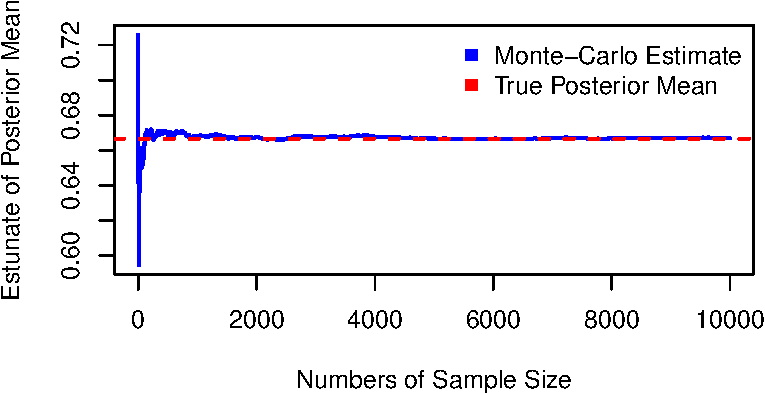
\includegraphics[keepaspectratio]{index_files/figure-pdf/fig-q1_mc_mean-1.pdf}}

}

\caption{\label{fig-q1_mc_mean}Convergence of True Posterior Mean by
Monte-Carlo method}

\end{figure}%

\begin{Shaded}
\begin{Highlighting}[]
\NormalTok{running\_sd }\OtherTok{=} \DecValTok{0}
\ControlFlowTok{for}\NormalTok{ (i }\ControlFlowTok{in} \DecValTok{1}\SpecialCharTok{:}\NormalTok{size)\{}
\NormalTok{  running\_sd[i] }\OtherTok{=} \FunctionTok{sd}\NormalTok{(rtheta[}\DecValTok{1}\SpecialCharTok{:}\NormalTok{i])}
\NormalTok{\}}

\FunctionTok{plot}\NormalTok{(running\_sd, }\AttributeTok{type=}\StringTok{\textquotesingle{}l\textquotesingle{}}\NormalTok{,}\AttributeTok{col=}\StringTok{"blue"}\NormalTok{,}\AttributeTok{lwd=}\DecValTok{2}\NormalTok{,}\AttributeTok{xlab =} \StringTok{"Numbers of Sample Size"}\NormalTok{, }\AttributeTok{ylab=}\StringTok{"Estunate of Posterior Standard Deviation"}\NormalTok{)}
\FunctionTok{abline}\NormalTok{(}\AttributeTok{h=}\NormalTok{sd\_true,}\AttributeTok{col=}\StringTok{"red"}\NormalTok{,}\AttributeTok{lwd=}\DecValTok{2}\NormalTok{,}\AttributeTok{lty=}\DecValTok{2}\NormalTok{)}
\FunctionTok{legend}\NormalTok{(}\StringTok{"topright"}\NormalTok{,}\AttributeTok{legend=}\FunctionTok{c}\NormalTok{(}\StringTok{"Monte{-}Carlo Estimate"}\NormalTok{,}\StringTok{"True Posterior Standard Deviation"}\NormalTok{),}\AttributeTok{col=}\FunctionTok{c}\NormalTok{(}\StringTok{"blue"}\NormalTok{,}\StringTok{"red"}\NormalTok{),}\AttributeTok{pch=}\DecValTok{15}\NormalTok{,}\AttributeTok{bty=}\StringTok{"n"}\NormalTok{)}
\end{Highlighting}
\end{Shaded}

\begin{figure}[H]

\centering{

\pandocbounded{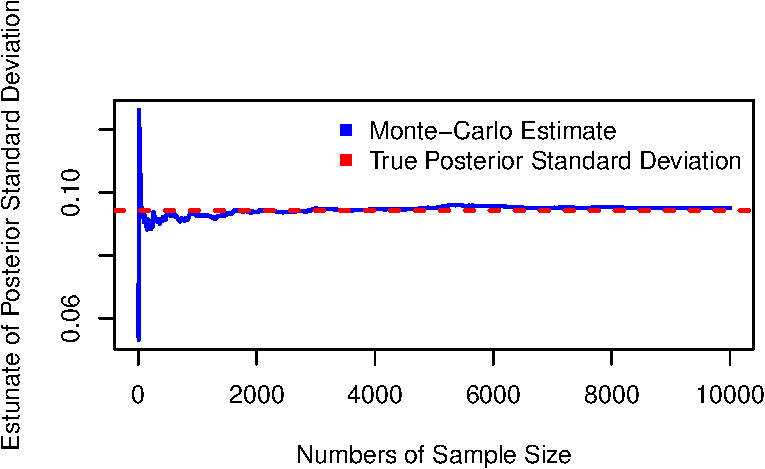
\includegraphics[keepaspectratio]{index_files/figure-pdf/fig-q1_mc_sd-1.pdf}}

}

\caption{\label{fig-q1_mc_sd}Convergence of True Posterior Standard
Deviation by Monte-Carlo method}

\end{figure}%

\subsubsection{Problem 1b)}\label{problem-1b}

In this task, we calculate the posterior probability
\(Pr(\theta<0.5|\textbf{y})\) by simulation, and compare the exact value
by \texttt{pbeta()}. The result shows that the simulated answer is
0.0478, and the exact value is 0.0466, simulated value is pretty close
to exact one.

\begin{Shaded}
\begin{Highlighting}[]
\NormalTok{nDraws }\OtherTok{=} \DecValTok{10000}
\FunctionTok{set.seed}\NormalTok{(}\DecValTok{42}\NormalTok{)}


\NormalTok{prob\_sim }\OtherTok{=} \FunctionTok{mean}\NormalTok{(}\FunctionTok{rbeta}\NormalTok{(nDraws,alpha\_post,beta\_post)}\SpecialCharTok{\textless{}=}\FloatTok{0.5}\NormalTok{)}
\NormalTok{prob\_true }\OtherTok{=} \FunctionTok{pbeta}\NormalTok{(}\FloatTok{0.5}\NormalTok{,alpha\_post,beta\_post)}

\CommentTok{\# prob\_sim = 0.0478}
\CommentTok{\# prob\_true ≈ 0.04656}
\end{Highlighting}
\end{Shaded}

\subsubsection{Problem 1c)}\label{problem-1c}

In this task, we simulate the posterior distribution of the log-odds
\(\phi = log(\frac{\theta}{1-\theta})\). the method \texttt{qlogis()}
can compute the data with log-odds transformation, which is equivalent
to \texttt{transformed\ =\ log(theta/(1-theta))}.

\begin{Shaded}
\begin{Highlighting}[]
\FunctionTok{set.seed}\NormalTok{(}\DecValTok{42}\NormalTok{)}
\NormalTok{theta\_original }\OtherTok{=} \FunctionTok{rbeta}\NormalTok{(size,alpha\_post,beta\_post)}
\NormalTok{theta\_trans }\OtherTok{=} \FunctionTok{qlogis}\NormalTok{(theta\_original)}

\FunctionTok{hist}\NormalTok{(theta\_trans,}\AttributeTok{xlab=}\StringTok{"log{-}odds theta"}\NormalTok{,}\AttributeTok{main=}\StringTok{""}\NormalTok{,}\AttributeTok{ylab=}\StringTok{"Density"}\NormalTok{)}
\end{Highlighting}
\end{Shaded}

\begin{figure}[H]

\centering{

\pandocbounded{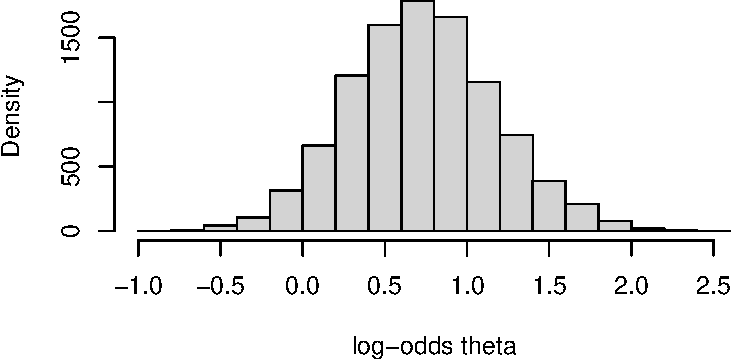
\includegraphics[keepaspectratio]{index_files/figure-pdf/fig-q1_hist-1.pdf}}

}

\caption{\label{fig-q1_hist}Histogram of log-odds theta}

\end{figure}%

\subsection{Problem 2}\label{problem-2}

In this task, we explore dataset \texttt{ericsson} on daily percentage
returns on Ericsson stock. Figure~\ref{fig-q2-standardized} shows the
distribution of standardized daily returns. Most values are centered
around zero, but the distribution exhibits heavy tails, with occasional
extreme negative returns.

\begin{Shaded}
\begin{Highlighting}[]
\FunctionTok{load}\NormalTok{(}\StringTok{"ericsson.RData"}\NormalTok{)}
\NormalTok{x }\OtherTok{=}\NormalTok{ (returns }\SpecialCharTok{{-}} \FunctionTok{mean}\NormalTok{(returns))}\SpecialCharTok{/}\FunctionTok{sd}\NormalTok{(returns)}
\FunctionTok{hist}\NormalTok{(x, }\DecValTok{30}\NormalTok{, }\AttributeTok{freq =} \ConstantTok{FALSE}\NormalTok{, }\AttributeTok{xlab =} \StringTok{"daily returns (standardized)"}\NormalTok{, }\AttributeTok{ylab =} \StringTok{"density"}\NormalTok{,}\AttributeTok{main =} \StringTok{""}\NormalTok{)}
\end{Highlighting}
\end{Shaded}

\begin{figure}[H]

\centering{

\pandocbounded{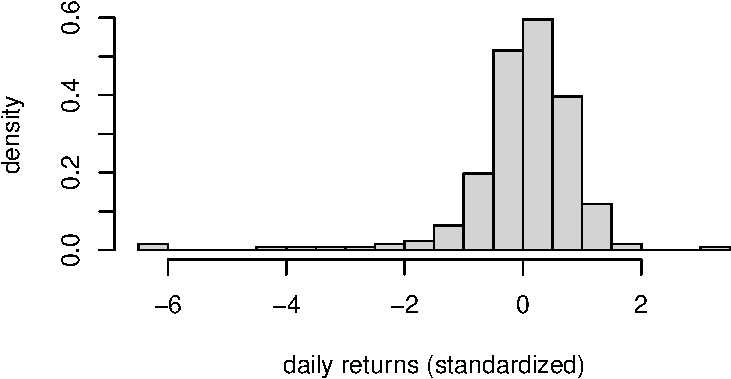
\includegraphics[keepaspectratio]{index_files/figure-pdf/fig-q2-standardized-1.pdf}}

}

\caption{\label{fig-q2-standardized}Histogram of standardized daily
returns}

\end{figure}%

\subsubsection{Problem 2a)}\label{problem-2a}

We computed the log-likelihood function over a series of candidate
degrees of freedom \(\nu\) and plotted the curve. In
Figure~\ref{fig-q2a}, we can notice that the log-likelihood curve
reaches its maximum value around 7, which implies that the maximum
likelihood estimate of the degree of freedon is \(\hat{\nu} \approx 7\).

\begin{Shaded}
\begin{Highlighting}[]
\NormalTok{nu\_potential }\OtherTok{=} \FunctionTok{seq}\NormalTok{(}\FloatTok{0.5}\NormalTok{,}\DecValTok{60}\NormalTok{,}\AttributeTok{by=}\FloatTok{0.1}\NormalTok{)}
\NormalTok{loglike }\OtherTok{=} \FunctionTok{numeric}\NormalTok{(}\FunctionTok{length}\NormalTok{(nu\_potential))}

\ControlFlowTok{for}\NormalTok{ (i }\ControlFlowTok{in} \FunctionTok{seq\_along}\NormalTok{(nu\_potential))\{}
\NormalTok{  loglike[i] }\OtherTok{=} \FunctionTok{sum}\NormalTok{(}\FunctionTok{dt}\NormalTok{(x,}\AttributeTok{df=}\NormalTok{nu\_potential[i],}\AttributeTok{log=}\ConstantTok{TRUE}\NormalTok{))}
\NormalTok{\}}

\FunctionTok{plot}\NormalTok{(nu\_potential,loglike,}\AttributeTok{type=}\StringTok{\textquotesingle{}l\textquotesingle{}}\NormalTok{,}\AttributeTok{xlab=}\StringTok{"potential nu values"}\NormalTok{,}\AttributeTok{ylab=}\StringTok{"log{-}likelihood"}\NormalTok{,}\AttributeTok{lwd=}\DecValTok{2}\NormalTok{)}

\NormalTok{nu\_mle }\OtherTok{=}\NormalTok{ nu\_potential[}\FunctionTok{which.max}\NormalTok{(loglike)]}
\CommentTok{\# nu\_mle = 7}
\FunctionTok{abline}\NormalTok{(}\AttributeTok{v=}\NormalTok{nu\_mle,}\AttributeTok{col=}\StringTok{"red"}\NormalTok{,}\AttributeTok{lty=}\DecValTok{2}\NormalTok{,}\AttributeTok{lwd=}\DecValTok{2}\NormalTok{)}
\end{Highlighting}
\end{Shaded}

\begin{figure}[H]

\centering{

\pandocbounded{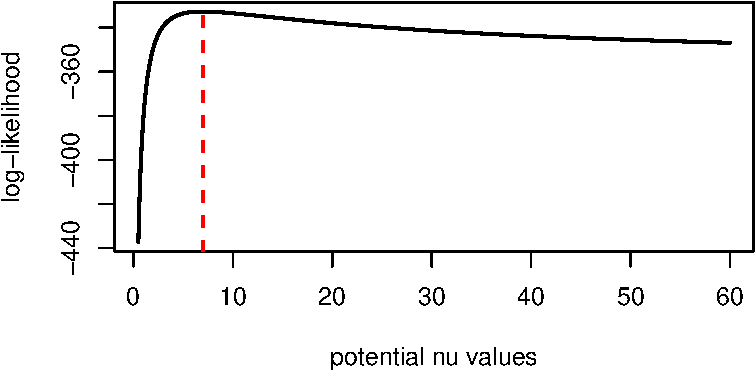
\includegraphics[keepaspectratio]{index_files/figure-pdf/fig-q2a-1.pdf}}

}

\caption{\label{fig-q2a}Curve of log-likelihood in potential degrees of
freedom nu}

\end{figure}%

\subsubsection{Problem 2b)}\label{problem-2b}

We plot the likelihood \(L(x_1,...,x_n|\nu)=\prod_ip(x_i|\nu)\) and
plotted the curve. in Figure~\ref{fig-q2b}, the red line and blue line
represent \(\nu = 1\) and \(\nu = 10\) respectively. The likelihood
peaks around \(\nu \approx 7\). Clearly, \(L(1)\) (also called Cauchy
Distribution) is obviously smaller than \(L(10)\), showing that the data
are heavy-tailed, but not as extreme as a Cauchy distribution.

\begin{Shaded}
\begin{Highlighting}[]
\NormalTok{nu\_potential }\OtherTok{=} \FunctionTok{seq}\NormalTok{(}\FloatTok{0.5}\NormalTok{,}\DecValTok{60}\NormalTok{,}\AttributeTok{by=}\FloatTok{0.1}\NormalTok{)}
\NormalTok{likelihood }\OtherTok{=} \FunctionTok{numeric}\NormalTok{(}\FunctionTok{length}\NormalTok{(nu\_potential))}
\ControlFlowTok{for}\NormalTok{ (i }\ControlFlowTok{in} \FunctionTok{seq\_along}\NormalTok{(likelihood))\{}
\NormalTok{  likelihood[i] }\OtherTok{=} \FunctionTok{prod}\NormalTok{(}\FunctionTok{dt}\NormalTok{(x,}\AttributeTok{df=}\NormalTok{nu\_potential[i],}\AttributeTok{log=}\ConstantTok{FALSE}\NormalTok{))}
\NormalTok{\}}
\FunctionTok{plot}\NormalTok{(nu\_potential,likelihood,}\AttributeTok{type=}\StringTok{\textquotesingle{}l\textquotesingle{}}\NormalTok{,}\AttributeTok{xlab=}\StringTok{"Potential nu values"}\NormalTok{,}\AttributeTok{ylab=}\StringTok{"Likelihood"}\NormalTok{,}\AttributeTok{lwd=}\DecValTok{2}\NormalTok{)}
\FunctionTok{abline}\NormalTok{(}\AttributeTok{v=}\DecValTok{1}\NormalTok{,}\AttributeTok{col=}\StringTok{"red"}\NormalTok{,}\AttributeTok{lty=}\DecValTok{2}\NormalTok{,}\AttributeTok{lwd=}\DecValTok{2}\NormalTok{)}
\FunctionTok{abline}\NormalTok{(}\AttributeTok{v=}\DecValTok{10}\NormalTok{,}\AttributeTok{col=}\StringTok{"blue"}\NormalTok{,}\AttributeTok{lty=}\DecValTok{2}\NormalTok{,}\AttributeTok{lwd=}\DecValTok{2}\NormalTok{)}
\FunctionTok{legend}\NormalTok{(}\StringTok{"topright"}\NormalTok{,}\FunctionTok{c}\NormalTok{(}\StringTok{"nu = 1"}\NormalTok{,}\StringTok{"nu = 10"}\NormalTok{),}\AttributeTok{col =} \FunctionTok{c}\NormalTok{(}\StringTok{"red"}\NormalTok{,}\StringTok{"blue"}\NormalTok{),}\AttributeTok{lty=}\DecValTok{2}\NormalTok{,}\AttributeTok{lwd=}\DecValTok{2}\NormalTok{)}
\end{Highlighting}
\end{Shaded}

\begin{figure}[H]

\centering{

\pandocbounded{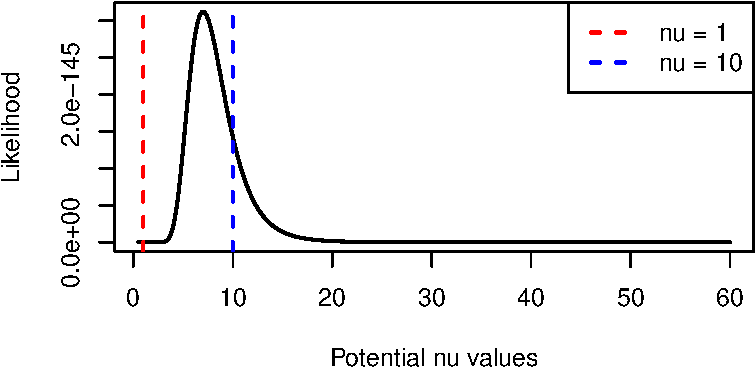
\includegraphics[keepaspectratio]{index_files/figure-pdf/fig-q2b-1.pdf}}

}

\caption{\label{fig-q2b}Curve of likelihood with respect to potential
degrees of freedom nu}

\end{figure}%

\subsection{Problem 2c)}\label{problem-2c}

In this step, we plot the logarithm of the posterior distribution for
\(\nu\), using
\[\log p(\nu \mid x_1,\dots,x_n) \;\propto\; \log p(x_1,\dots,x_n \mid \nu) + \log p(\nu),\]

we evaluate the log-likelihood over a series of candidate values of
\(nu\) and add the log prior. Note that the prior is
\(\nu \sim \text{Exponential}(0.25)\) with the rate parameterization.
The resulting curve (Figure~\ref{fig-q2c}) shows that the log-posterior
peaks around \(\nu \approx7\).

\begin{Shaded}
\begin{Highlighting}[]
\NormalTok{nu\_potential }\OtherTok{=} \FunctionTok{seq}\NormalTok{(}\FloatTok{0.5}\NormalTok{,}\DecValTok{60}\NormalTok{,}\AttributeTok{by=}\FloatTok{0.1}\NormalTok{)}
\NormalTok{log\_post}\OtherTok{=} \FunctionTok{numeric}\NormalTok{(}\FunctionTok{length}\NormalTok{(nu\_potential))}
\ControlFlowTok{for}\NormalTok{ (i }\ControlFlowTok{in} \FunctionTok{seq\_along}\NormalTok{(nu\_potential))\{}
\NormalTok{  nu }\OtherTok{=}\NormalTok{ nu\_potential[i]}
\NormalTok{  logprior }\OtherTok{=} \FunctionTok{dexp}\NormalTok{(nu,}\AttributeTok{rate=}\FloatTok{0.25}\NormalTok{,}\AttributeTok{log=}\ConstantTok{TRUE}\NormalTok{)}
\NormalTok{  loglike }\OtherTok{=} \FunctionTok{sum}\NormalTok{(}\FunctionTok{dt}\NormalTok{(x,}\AttributeTok{df=}\NormalTok{nu,}\AttributeTok{log=}\ConstantTok{TRUE}\NormalTok{))}
\NormalTok{  log\_post[i] }\OtherTok{=}\NormalTok{ loglike }\SpecialCharTok{+}\NormalTok{logprior}
\NormalTok{\}}
\FunctionTok{plot}\NormalTok{(nu\_potential,log\_post,}\AttributeTok{type=}\StringTok{\textquotesingle{}l\textquotesingle{}}\NormalTok{,}\AttributeTok{xlab=}\StringTok{\textquotesingle{}nu values\textquotesingle{}}\NormalTok{,}\AttributeTok{ylab =} \StringTok{\textquotesingle{}log{-}posterior\textquotesingle{}}\NormalTok{,}\AttributeTok{lwd=}\DecValTok{2}\NormalTok{)}
\end{Highlighting}
\end{Shaded}

\begin{figure}[H]

\centering{

\pandocbounded{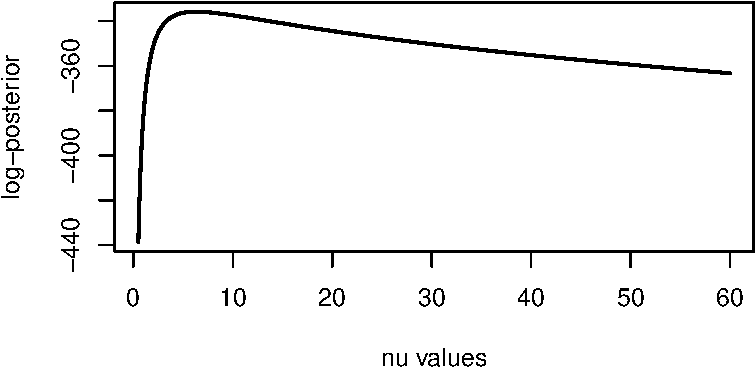
\includegraphics[keepaspectratio]{index_files/figure-pdf/fig-q2c-1.pdf}}

}

\caption{\label{fig-q2c}Curve of logarithm of the posterior distribution
for nu}

\end{figure}%

\subsection{Problem 2d)}\label{problem-2d}

In order to plot the posterior of distribution of \(nu\), we firstly
transform the log-posterior to unnormalized posterior as
\[p(\nu \mid x_1,\dots,x_n) \;\propto\;  p(x_1,\dots,x_n \mid \nu) p(\nu)\]

Then, we need to normalize the posterior as a true probability density
function:
\[p(\nu|x_1,...,x_n)=\frac{p(x_1,...,x_n|\nu)p(\nu)}{\int_0^{\infty}p(x_1,...,x_n|\nu)p(\nu)d\nu}\]
we can use Riemann approximation to calculate the integral:
\[p(\nu|x_1,...,x_n)\approx \frac{p(x_1,...,x_n|\nu_i)p(\nu_i)}{\sum_j p(x_1,...,x_n|\nu_j)p(\nu_j)\Delta\nu}\]
where \(\Delta\nu\) means the length of each step.

Figure~\ref{fig-q2d} The blue line and orange line represents the
posterior and prior respectively.

\begin{Shaded}
\begin{Highlighting}[]
\NormalTok{unnormalized\_posterior }\OtherTok{=} \FunctionTok{exp}\NormalTok{(log\_post)}
\NormalTok{distance }\OtherTok{=} \FloatTok{0.1}
\NormalTok{posterior }\OtherTok{=}\NormalTok{ unnormalized\_posterior}\SpecialCharTok{/}\NormalTok{(}\FunctionTok{sum}\NormalTok{(unnormalized\_posterior)}\SpecialCharTok{*}\NormalTok{distance)}
\FunctionTok{plot}\NormalTok{(nu\_potential,posterior, }\AttributeTok{type=}\StringTok{"l"}\NormalTok{,}\AttributeTok{col =} \StringTok{\textquotesingle{}blue\textquotesingle{}}\NormalTok{,}\AttributeTok{xlab=}\StringTok{"nu"}\NormalTok{,}\AttributeTok{ylab=}\StringTok{"density"}\NormalTok{,}\AttributeTok{lwd=}\DecValTok{2}\NormalTok{)}
\FunctionTok{lines}\NormalTok{(nu\_potential,}\FunctionTok{dexp}\NormalTok{(nu\_potential,}\AttributeTok{rate=}\FloatTok{0.25}\NormalTok{),}\AttributeTok{col=}\StringTok{"orange"}\NormalTok{,}\AttributeTok{lwd=}\DecValTok{2}\NormalTok{)}
\FunctionTok{legend}\NormalTok{(}\StringTok{"topright"}\NormalTok{,}\FunctionTok{c}\NormalTok{(}\StringTok{"posterior"}\NormalTok{,}\StringTok{"prior"}\NormalTok{),}\AttributeTok{col=}\FunctionTok{c}\NormalTok{(}\StringTok{"blue"}\NormalTok{,}\StringTok{"orange"}\NormalTok{),}\AttributeTok{lty=}\DecValTok{1}\NormalTok{,}\AttributeTok{lwd=}\DecValTok{4}\NormalTok{)}
\end{Highlighting}
\end{Shaded}

\begin{figure}[H]

\centering{

\pandocbounded{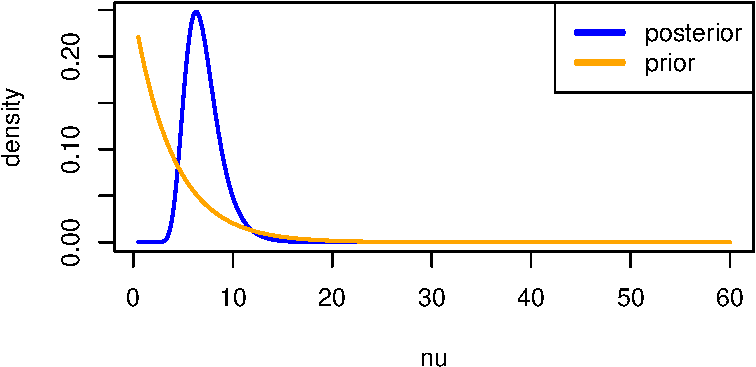
\includegraphics[keepaspectratio]{index_files/figure-pdf/fig-q2d-1.pdf}}

}

\caption{\label{fig-q2d}Posterior and Prior Distributions of the Degrees
of Freedom nu}

\end{figure}%

\subsubsection{Problem 2e)}\label{problem-2e}

The defination of Posterior mean is
\[\mathbb{E}(\nu|x_1,...,x_n)=\int_0^{\infty}\nu p(\nu | x_1,...,x_n)d\nu\]
where \(p(\nu|x_1,...,x_n)\) is normalized posterior distribution. We
use Riemann sum, same as Problem 2d, to approximate the integral:
\[\mathbb{E}(\nu|x_1,...,x_n)\approx \sum_{i=1}^m\nu_i p(\nu_i|x_1,...,x_n)\Delta\nu\]
and the posterior mean of \(\nu = 7.0807\)

\begin{Shaded}
\begin{Highlighting}[]
\NormalTok{post\_mean }\OtherTok{=} \FunctionTok{sum}\NormalTok{(nu\_potential}\SpecialCharTok{*}\NormalTok{posterior) }\SpecialCharTok{*} \FloatTok{0.1}
\end{Highlighting}
\end{Shaded}

\subsubsection{Load packages}\label{load-packages}

\begin{Shaded}
\begin{Highlighting}[]
\FunctionTok{library}\NormalTok{(mvtnorm)      }\CommentTok{\# package with multivariate normal density}
\FunctionTok{library}\NormalTok{(latex2exp)    }\CommentTok{\# latex maths in plots}
\end{Highlighting}
\end{Shaded}

\subsection{Problem 3a)}\label{problem-3a}

The Gamma prior is conjugate to possion model. We choose rate
parameterization for gamma distribution. The posterior distribution is
\(p(\theta|x_1,...x_n) \sim Gamma(\alpha+n\bar{x}, \beta+n)\) where
\(\alpha=7\), \(\beta=2\) from prior information.

\begin{Shaded}
\begin{Highlighting}[]
\DocumentationTok{\#\# likelihood sample}
\NormalTok{sample\_x }\OtherTok{=} \FunctionTok{c}\NormalTok{(}\DecValTok{3}\NormalTok{, }\DecValTok{5}\NormalTok{, }\DecValTok{4}\NormalTok{, }\DecValTok{3}\NormalTok{, }\DecValTok{6}\NormalTok{, }\DecValTok{8}\NormalTok{, }\DecValTok{6}\NormalTok{, }\DecValTok{1}\NormalTok{, }\DecValTok{14}\NormalTok{, }\DecValTok{3}\NormalTok{)}
\NormalTok{sample\_x\_size }\OtherTok{=} \FunctionTok{length}\NormalTok{(sample\_x)}
\NormalTok{sample\_x\_mean }\OtherTok{=} \FunctionTok{mean}\NormalTok{(sample\_x)}
\end{Highlighting}
\end{Shaded}

\begin{Shaded}
\begin{Highlighting}[]
\DocumentationTok{\#\# parameters for prior}
\NormalTok{alpha }\OtherTok{=} \DecValTok{7}
\NormalTok{beta }\OtherTok{=} \DecValTok{2}

\CommentTok{\# posterior simulation}
\NormalTok{n\_draw }\OtherTok{=} \DecValTok{10000}
\NormalTok{theta\_sample }\OtherTok{=} \FunctionTok{rgamma}\NormalTok{(n\_draw, alpha}\SpecialCharTok{+}\FunctionTok{sum}\NormalTok{(sample\_x), beta}\SpecialCharTok{+}\NormalTok{sample\_x\_size)}

\FunctionTok{hist}\NormalTok{(theta\_sample, }\AttributeTok{breaks =} \DecValTok{50}\NormalTok{, }\AttributeTok{probability =} \ConstantTok{TRUE}\NormalTok{,}
     \AttributeTok{col =} \StringTok{"lightgray"}\NormalTok{, }\AttributeTok{border =} \StringTok{"white"}\NormalTok{,}
     \AttributeTok{main =} \StringTok{"Gamma Posterior Simulation"}\NormalTok{,}
     \AttributeTok{xlab =} \FunctionTok{expression}\NormalTok{(theta))}
\end{Highlighting}
\end{Shaded}

\pandocbounded{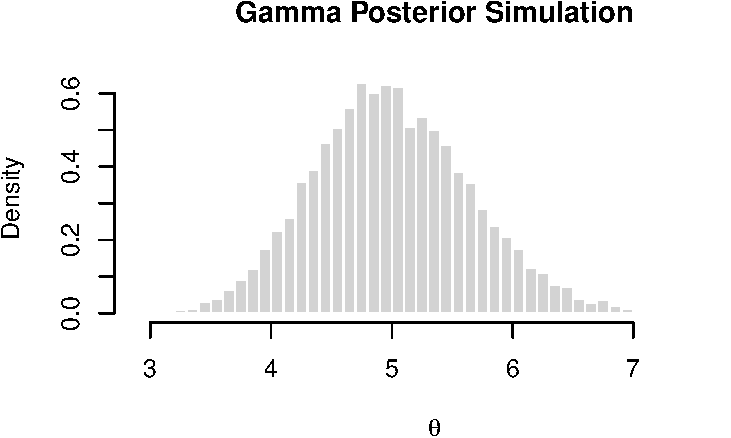
\includegraphics[keepaspectratio]{index_files/figure-pdf/unnamed-chunk-14-1.pdf}}

\begin{Shaded}
\begin{Highlighting}[]
\DocumentationTok{\#\# get all draw over 8}
\NormalTok{theta\_sample\_over\_8 }\OtherTok{=}\NormalTok{ theta\_sample }\SpecialCharTok{\textgreater{}} \DecValTok{8}
\DocumentationTok{\#\# calculate prob of theta\textgreater{}8 by using event\_size/sample\_size}
\FunctionTok{sum}\NormalTok{(theta\_sample\_over\_8)}\SpecialCharTok{/}\NormalTok{n\_draw}
\end{Highlighting}
\end{Shaded}

\begin{verbatim}
[1] 0
\end{verbatim}

\begin{Shaded}
\begin{Highlighting}[]
\CommentTok{\# use gamma cdf to get prob of over 8}
\FunctionTok{pgamma}\NormalTok{(}\DecValTok{8}\NormalTok{, alpha}\SpecialCharTok{+}\FunctionTok{sum}\NormalTok{(sample\_x), beta}\SpecialCharTok{+}\NormalTok{sample\_x\_size, }\AttributeTok{lower.tail =} \ConstantTok{FALSE}\NormalTok{)}
\end{Highlighting}
\end{Shaded}

\begin{verbatim}
[1] 3.291869e-05
\end{verbatim}

\begin{Shaded}
\begin{Highlighting}[]
\CommentTok{\# check gamma pdf}
\CommentTok{\# curve(dgamma(x, alpha+sum(sample\_x), beta+sample\_x\_size), from=0, to=9, ylab="gamma pdf")}
\end{Highlighting}
\end{Shaded}

\subsection{Problem 3b)}\label{problem-3b}

\begin{Shaded}
\begin{Highlighting}[]
\CommentTok{\# predictive simulation}
\NormalTok{predDraws }\OtherTok{=} \FunctionTok{rnbinom}\NormalTok{(n\_draw, alpha}\SpecialCharTok{+}\FunctionTok{sum}\NormalTok{(sample\_x), (beta}\SpecialCharTok{+}\NormalTok{sample\_x\_size)}\SpecialCharTok{/}\NormalTok{(beta}\SpecialCharTok{+}\NormalTok{sample\_x\_size}\SpecialCharTok{+}\DecValTok{1}\NormalTok{))}
\FunctionTok{hist}\NormalTok{(predDraws,}
     \AttributeTok{xlab =} \StringTok{"Max weight on a future day"}\NormalTok{, }\AttributeTok{ylab =} \StringTok{"Predictive density"}\NormalTok{, }
     \AttributeTok{main =} \StringTok{"Predictive density max weight {-} single day"}\NormalTok{, }\AttributeTok{col =} \StringTok{"lightgray"}\NormalTok{, }\AttributeTok{border =} \StringTok{"white"}\NormalTok{)}
\end{Highlighting}
\end{Shaded}

\pandocbounded{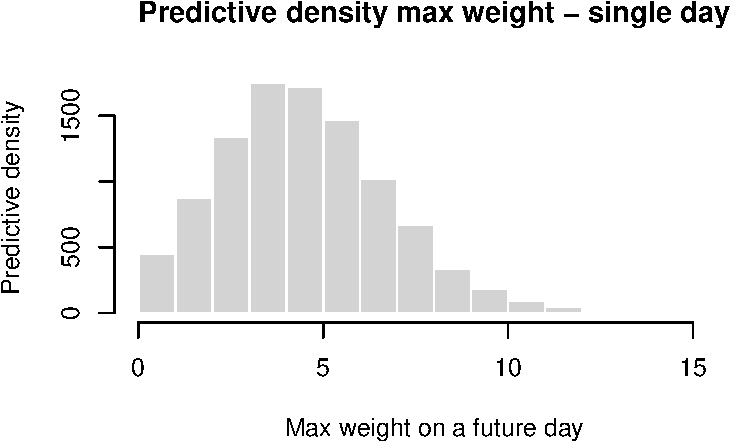
\includegraphics[keepaspectratio]{index_files/figure-pdf/unnamed-chunk-15-1.pdf}}

\begin{Shaded}
\begin{Highlighting}[]
\DocumentationTok{\#\# get all draw over 8}
\NormalTok{temp }\OtherTok{=}\NormalTok{ predDraws }\SpecialCharTok{\textgreater{}=} \DecValTok{8}
\DocumentationTok{\#\# calculate prob of theta\textgreater{}=8 by using event\_size/sample\_size}
\FunctionTok{mean}\NormalTok{(temp)}
\end{Highlighting}
\end{Shaded}

\begin{verbatim}
[1] 0.1369
\end{verbatim}

\begin{Shaded}
\begin{Highlighting}[]
\CommentTok{\# use gamma cdf to get prob of over 8}
\CommentTok{\# negbinomial is discrete, cdf \textless{}= x, so using \textgreater{} 7}
\FunctionTok{pnbinom}\NormalTok{(}\DecValTok{7}\NormalTok{, alpha}\SpecialCharTok{+}\FunctionTok{sum}\NormalTok{(sample\_x), (beta}\SpecialCharTok{+}\NormalTok{sample\_x\_size)}\SpecialCharTok{/}\NormalTok{(beta}\SpecialCharTok{+}\NormalTok{sample\_x\_size}\SpecialCharTok{+}\DecValTok{1}\NormalTok{), }\AttributeTok{lower.tail =} \ConstantTok{FALSE}\NormalTok{)}
\end{Highlighting}
\end{Shaded}

\begin{verbatim}
[1] 0.141594
\end{verbatim}

\subsection{Problem 3c)}\label{problem-3c}

The utility function is a function of random varibable \(X_{11}\). And
\(a_{11}\) is treated as a constant. \begin{equation} 
U = \begin{cases}
10a_{11} & \text{if} X_{11} \geq a_{11}, \\
10X_{11} - 7(a_{11}-X_{11}) & \text{if} X_{11} < a_{11}
\end{cases}
\end{equation}

With simplification, it should be \begin{equation} 
U = \begin{cases}
10a_{11} & \text{if } X_{11} \geq a_{11}\\
17X_{11} - 7a_{11} & \text{if } X_{11} < a_{11}
\end{cases}
\end{equation} The expected value of utility function is
\(E(U)=10a_{11}*Pr(X_{11} \geq a_{11}|a_{11},x_{1}...,x_{10}) +E(17X_{11}-7a_{11}|X_{11}<a_{11})*Pr(X_{11} < a_{11}|a_{11},x_{1}...,x_{10})\)
It is required to find the maximal value of expected utility. The
uncertainty comes from demand \(X_{11}\) and storage \(a_{11}\). The
predictive distribution of \(X_{11}\) is from simulation. And only using
\(a_{11}\) as varibale and get the maximizer in expected utility.

\begin{Shaded}
\begin{Highlighting}[]
\NormalTok{aGrid }\OtherTok{=} \FunctionTok{seq}\NormalTok{(}\DecValTok{0}\NormalTok{, }\DecValTok{15}\NormalTok{, }\AttributeTok{length =} \DecValTok{1000}\NormalTok{)}
\NormalTok{EL }\OtherTok{=} \FunctionTok{rep}\NormalTok{(}\FunctionTok{length}\NormalTok{(aGrid))}
\ControlFlowTok{for}\NormalTok{ (i }\ControlFlowTok{in} \DecValTok{1}\SpecialCharTok{:}\FunctionTok{length}\NormalTok{(aGrid))\{}
\NormalTok{  a }\OtherTok{=}\NormalTok{ aGrid[i]}
\NormalTok{  p }\OtherTok{=} \FunctionTok{mean}\NormalTok{(predDraws }\SpecialCharTok{\textgreater{}=}\NormalTok{ a)}
  
\NormalTok{  EL[i] }\OtherTok{=} \DecValTok{10}\SpecialCharTok{*}\NormalTok{a}\SpecialCharTok{*}\NormalTok{p }\SpecialCharTok{+}\NormalTok{(}\DecValTok{17}\SpecialCharTok{*}\FunctionTok{mean}\NormalTok{(predDraws[predDraws}\SpecialCharTok{\textless{}}\NormalTok{a])}\SpecialCharTok{{-}}\DecValTok{7}\SpecialCharTok{*}\NormalTok{a)}\SpecialCharTok{*}\NormalTok{(}\DecValTok{1}\SpecialCharTok{{-}}\NormalTok{p)}
\NormalTok{\}}
\FunctionTok{plot}\NormalTok{(aGrid, EL, }\AttributeTok{xlab =} \StringTok{"storage, a"}\NormalTok{, }\AttributeTok{ylab =} \StringTok{"Expected Utility"}\NormalTok{, }\AttributeTok{type =} \StringTok{"l"}\NormalTok{, }
     \AttributeTok{lwd =} \DecValTok{3}\NormalTok{, }\AttributeTok{col =} \StringTok{"lightgray"}\NormalTok{)}
\FunctionTok{abline}\NormalTok{(}\AttributeTok{v =}\NormalTok{ aGrid[}\FunctionTok{which.max}\NormalTok{(EL)], }\AttributeTok{lty =} \StringTok{"dotted"}\NormalTok{)}
\end{Highlighting}
\end{Shaded}

\pandocbounded{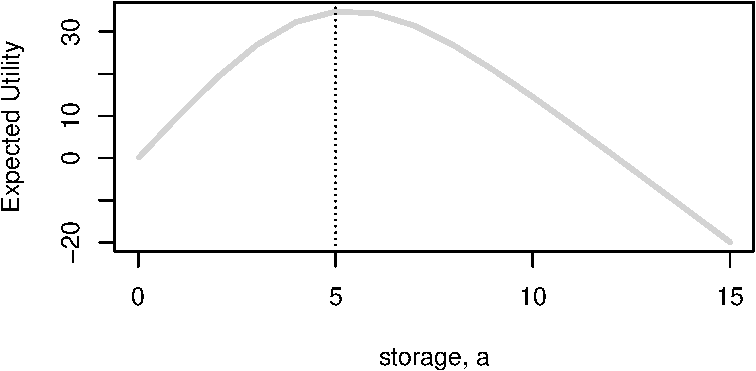
\includegraphics[keepaspectratio]{index_files/figure-pdf/unnamed-chunk-16-1.pdf}}

\begin{Shaded}
\begin{Highlighting}[]
\NormalTok{maximizer }\OtherTok{=}\NormalTok{ aGrid[}\FunctionTok{which.max}\NormalTok{(EL)]}
\NormalTok{maximizer}
\end{Highlighting}
\end{Shaded}

\begin{verbatim}
[1] 5
\end{verbatim}

\subsection{Problem 4}\label{problem-4}

Given information:

\[
temp = \beta_0 + \beta_1*time + \beta_2*time^2 + \epsilon, \ \epsilon\sim N(0, \sigma^2)
\]

\begin{Shaded}
\begin{Highlighting}[]
\CommentTok{\#install.packages("remotes")              \# Uncomment this the first time}
\FunctionTok{library}\NormalTok{(remotes)}
\CommentTok{\#install\_github("StatisticsSU/SUdatasets")  \# Uncomment this the first time}
\FunctionTok{library}\NormalTok{(SUdatasets)}
\FunctionTok{library}\NormalTok{(mvtnorm)}
\FunctionTok{library}\NormalTok{(ggplot2)}
\FunctionTok{head}\NormalTok{(tempLinkoping)}
\end{Highlighting}
\end{Shaded}

\begin{verbatim}
         time  temp
1 0.002732240   0.1
2 0.005464481  -4.5
3 0.008196721  -6.3
4 0.010928962  -9.6
5 0.013661202  -9.9
6 0.016393443 -17.1
\end{verbatim}

\begin{Shaded}
\begin{Highlighting}[]
\FunctionTok{summary}\NormalTok{(tempLinkoping)}
\end{Highlighting}
\end{Shaded}

\begin{verbatim}
      time               temp        
 Min.   :0.002732   Min.   :-17.100  
 1st Qu.:0.252049   1st Qu.:  1.925  
 Median :0.501366   Median :  6.900  
 Mean   :0.501366   Mean   :  7.524  
 3rd Qu.:0.750683   3rd Qu.: 14.575  
 Max.   :1.000000   Max.   : 23.100  
\end{verbatim}

\begin{Shaded}
\begin{Highlighting}[]
\FunctionTok{cat}\NormalTok{(}\StringTok{"The dataset contains"}\NormalTok{, }\FunctionTok{length}\NormalTok{(tempLinkoping}\SpecialCharTok{$}\NormalTok{time), }\StringTok{"observations."}\NormalTok{)}
\end{Highlighting}
\end{Shaded}

\begin{verbatim}
The dataset contains 366 observations.
\end{verbatim}

\subsubsection{4a) Determine a suitable prior
distribution}\label{a-determine-a-suitable-prior-distribution}

Given prior information:

\[
\boldsymbol{\beta} \vert \sigma^2 \sim N(\boldsymbol{\mu}_0,\sigma^2\boldsymbol{\Omega}_0^{-1}) 
\]

\[
\sigma^2 \sim \mathrm{inv-}\chi^2(\nu_0, \sigma_0^2)
\] The following figure shows the regression curves simulated from a
beta prior with \(\mu_0 (10, 100, -100)^T\). From
Figure~\ref{fig-reg-prior}, most of the temperatures variate above 0
degree which is higher than my belief of Linkoping's temperatures.

\begin{Shaded}
\begin{Highlighting}[]
\CommentTok{\#beta prior \textasciitilde{} normal}
\NormalTok{mu0 }\OtherTok{=} \FunctionTok{c}\NormalTok{(}\DecValTok{10}\NormalTok{,}\DecValTok{100}\NormalTok{,}\SpecialCharTok{{-}}\DecValTok{100}\NormalTok{)}
\NormalTok{sigma\_matrix0 }\OtherTok{=} \FloatTok{0.01}\SpecialCharTok{*}\FunctionTok{diag}\NormalTok{(}\DecValTok{3}\NormalTok{)}

\CommentTok{\#sigma\_sq prior \textasciitilde{} inv{-}x\^{}2 }
\NormalTok{nu0 }\OtherTok{=} \DecValTok{3}
\NormalTok{sigma0\_sq }\OtherTok{=} \DecValTok{1}

\CommentTok{\#store simulated betas, sigma\^{}2 and temps}
\NormalTok{m }\OtherTok{=} \DecValTok{200}
\NormalTok{time\_grid }\OtherTok{=}\NormalTok{tempLinkoping}\SpecialCharTok{$}\NormalTok{time}
\NormalTok{temp\_vals }\OtherTok{=} \FunctionTok{matrix}\NormalTok{(}\ConstantTok{NA}\NormalTok{, }\AttributeTok{nrow=}\NormalTok{m, }\AttributeTok{ncol=}\FunctionTok{length}\NormalTok{(time\_grid))}

\CommentTok{\# Simulator for the scaled inverse Chi{-}square distribution}
\NormalTok{rScaledInvChi2 }\OtherTok{\textless{}{-}} \ControlFlowTok{function}\NormalTok{(n, v\_0, sigma2\_0)\{}
  \FunctionTok{return}\NormalTok{((v\_0}\SpecialCharTok{*}\NormalTok{sigma2\_0)}\SpecialCharTok{/}\FunctionTok{rchisq}\NormalTok{(n, }\AttributeTok{df =}\NormalTok{ v\_0))}
\NormalTok{\}}

\CommentTok{\#simulated sigma\_prior and beta\_prior}
\FunctionTok{set.seed}\NormalTok{(}\DecValTok{42}\NormalTok{)}

\NormalTok{sigma\_sq\_draws }\OtherTok{=} \FunctionTok{rScaledInvChi2}\NormalTok{(m, }\AttributeTok{v\_0=}\NormalTok{nu0, }\AttributeTok{sigma2\_0 =}\NormalTok{ sigma0\_sq)}

\ControlFlowTok{for}\NormalTok{ (i }\ControlFlowTok{in} \DecValTok{1}\SpecialCharTok{:}\NormalTok{m)\{}
\NormalTok{  sigma\_sq\_i }\OtherTok{=}\NormalTok{ sigma\_sq\_draws[i]}
\NormalTok{  betas\_i }\OtherTok{=} \FunctionTok{rmvnorm}\NormalTok{(}\DecValTok{1}\NormalTok{, }\AttributeTok{mean=}\NormalTok{mu0, }\AttributeTok{sigma=}\NormalTok{(sigma\_sq\_i}\SpecialCharTok{*}\FunctionTok{solve}\NormalTok{(sigma\_matrix0)))}
\NormalTok{  temp\_vals[i, ] }\OtherTok{=}\NormalTok{ betas\_i[}\DecValTok{1}\NormalTok{] }\SpecialCharTok{+}\NormalTok{ betas\_i[}\DecValTok{2}\NormalTok{]}\SpecialCharTok{*}\NormalTok{time\_grid }\SpecialCharTok{+}\NormalTok{ betas\_i[}\DecValTok{3}\NormalTok{]}\SpecialCharTok{*}\NormalTok{time\_grid}\SpecialCharTok{\^{}}\DecValTok{2}
\NormalTok{\}}

\FunctionTok{plot}\NormalTok{(}
  \ConstantTok{NA}\NormalTok{, }\ConstantTok{NA}\NormalTok{,}
  \AttributeTok{xlim =} \FunctionTok{c}\NormalTok{(}\DecValTok{0}\NormalTok{, }\DecValTok{1}\NormalTok{),}
  \AttributeTok{ylim =} \FunctionTok{range}\NormalTok{(temp\_vals),}
  \AttributeTok{xlab =} \StringTok{"Normalized Time"}\NormalTok{,}
  \AttributeTok{ylab =} \StringTok{"Temperatures"}\NormalTok{,}
  \AttributeTok{main =} \StringTok{"Simulated Regression Curves from Prior"}
\NormalTok{)}

\CommentTok{\# Now overlay all the curves}
\ControlFlowTok{for}\NormalTok{ (i }\ControlFlowTok{in} \DecValTok{1}\SpecialCharTok{:}\FunctionTok{nrow}\NormalTok{(temp\_vals)) \{}
  \FunctionTok{lines}\NormalTok{(time\_grid, temp\_vals[i, ], }\AttributeTok{col =} \FunctionTok{rgb}\NormalTok{(}\DecValTok{0}\NormalTok{, }\DecValTok{0}\NormalTok{, }\DecValTok{0}\NormalTok{, }\AttributeTok{alpha =} \FloatTok{0.3}\NormalTok{))}
\NormalTok{\}}
\end{Highlighting}
\end{Shaded}

\begin{figure}[H]

\centering{

\pandocbounded{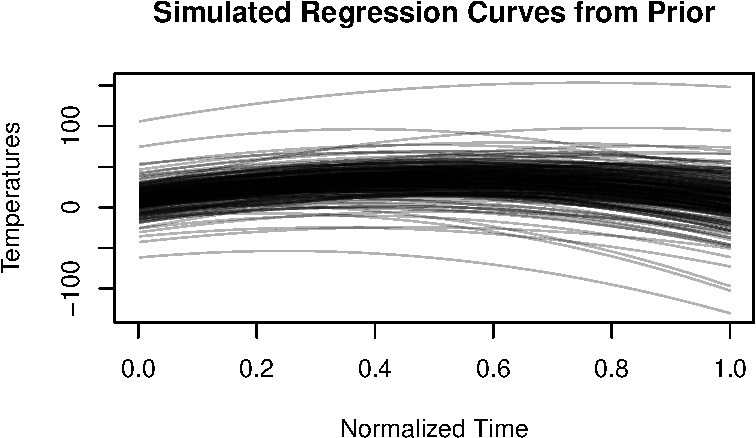
\includegraphics[keepaspectratio]{index_files/figure-pdf/fig-reg-prior-1.pdf}}

}

\caption{\label{fig-reg-prior}Simulated Regression Curves from Prior}

\end{figure}%

The original prior information is much higher than my belief.
Figure~\ref{fig-reg-prior-new} is the regression curves plot with
updated prior information \(\mu_0 (5, 70, -70)^T\), it clearly shows
that half of the simulated temperature curves variate below 0 degree
which satisfies my beliefs of temperature variation in Linkoping.

\begin{Shaded}
\begin{Highlighting}[]
\CommentTok{\#beta prior \textasciitilde{} normal updated}
\NormalTok{mu0 }\OtherTok{=} \FunctionTok{c}\NormalTok{(}\DecValTok{5}\NormalTok{,}\DecValTok{70}\NormalTok{,}\SpecialCharTok{{-}}\DecValTok{70}\NormalTok{)}
\NormalTok{Omega\_matrix0 }\OtherTok{=} \FloatTok{0.01}\SpecialCharTok{*}\FunctionTok{diag}\NormalTok{(}\DecValTok{3}\NormalTok{)}

\CommentTok{\#sigma\_sq prior \textasciitilde{} inv{-}x\^{}2 }
\NormalTok{nu0 }\OtherTok{=} \DecValTok{3}
\NormalTok{sigma0\_sq }\OtherTok{=} \DecValTok{1}

\CommentTok{\#store simulated betas, sigma\^{}2 and temps}
\NormalTok{m }\OtherTok{=} \DecValTok{200}
\NormalTok{time\_grid }\OtherTok{=} \FunctionTok{seq}\NormalTok{(}\DecValTok{0}\NormalTok{, }\DecValTok{1}\NormalTok{, }\AttributeTok{length.out=}\DecValTok{366}\NormalTok{)}
\NormalTok{temp\_vals }\OtherTok{=} \FunctionTok{matrix}\NormalTok{(}\ConstantTok{NA}\NormalTok{, }\AttributeTok{nrow=}\NormalTok{m, }\AttributeTok{ncol=}\FunctionTok{length}\NormalTok{(time\_grid))}

\CommentTok{\# Simulator for the scaled inverse Chi{-}square distribution}
\NormalTok{rScaledInvChi2 }\OtherTok{\textless{}{-}} \ControlFlowTok{function}\NormalTok{(n, v\_0, sigma2\_0)\{}
  \FunctionTok{return}\NormalTok{((v\_0}\SpecialCharTok{*}\NormalTok{sigma2\_0)}\SpecialCharTok{/}\FunctionTok{rchisq}\NormalTok{(n, }\AttributeTok{df =}\NormalTok{ v\_0))}
\NormalTok{\}}

\CommentTok{\#simulated sigma\_prior and beta\_prior}
\FunctionTok{set.seed}\NormalTok{(}\DecValTok{42}\NormalTok{)}

\NormalTok{sigma\_sq\_draws }\OtherTok{=} \FunctionTok{rScaledInvChi2}\NormalTok{(m, }\AttributeTok{v\_0=}\NormalTok{nu0, }\AttributeTok{sigma2\_0 =}\NormalTok{ sigma0\_sq)}

\ControlFlowTok{for}\NormalTok{ (i }\ControlFlowTok{in} \DecValTok{1}\SpecialCharTok{:}\NormalTok{m)\{}
\NormalTok{  sigma\_sq\_i }\OtherTok{=}\NormalTok{ sigma\_sq\_draws[i]}
\NormalTok{  betas\_i }\OtherTok{=} \FunctionTok{rmvnorm}\NormalTok{(}\DecValTok{1}\NormalTok{, }\AttributeTok{mean=}\NormalTok{mu0, }\AttributeTok{sigma=}\NormalTok{(sigma\_sq\_i}\SpecialCharTok{*}\FunctionTok{solve}\NormalTok{(Omega\_matrix0)))}
\NormalTok{  temp\_vals[i, ] }\OtherTok{=}\NormalTok{ betas\_i[}\DecValTok{1}\NormalTok{] }\SpecialCharTok{+}\NormalTok{ betas\_i[}\DecValTok{2}\NormalTok{]}\SpecialCharTok{*}\NormalTok{time\_grid }\SpecialCharTok{+}\NormalTok{ betas\_i[}\DecValTok{3}\NormalTok{]}\SpecialCharTok{*}\NormalTok{time\_grid}\SpecialCharTok{\^{}}\DecValTok{2}
\NormalTok{\}}

\FunctionTok{plot}\NormalTok{(}
  \ConstantTok{NA}\NormalTok{, }\ConstantTok{NA}\NormalTok{,}
  \AttributeTok{xlim =} \FunctionTok{c}\NormalTok{(}\DecValTok{0}\NormalTok{, }\DecValTok{1}\NormalTok{),}
  \AttributeTok{ylim =} \FunctionTok{range}\NormalTok{(temp\_vals),}
  \AttributeTok{xlab =} \StringTok{"Normalized Time"}\NormalTok{,}
  \AttributeTok{ylab =} \StringTok{"Temperatures"}\NormalTok{,}
  \AttributeTok{main =} \StringTok{"Simulated Regression Curves from Updated Prior"}
\NormalTok{)}

\CommentTok{\# Now overlay all the curves}
\ControlFlowTok{for}\NormalTok{ (i }\ControlFlowTok{in} \DecValTok{1}\SpecialCharTok{:}\FunctionTok{nrow}\NormalTok{(temp\_vals)) \{}
  \FunctionTok{lines}\NormalTok{(time\_grid, temp\_vals[i, ], }\AttributeTok{col =} \FunctionTok{rgb}\NormalTok{(}\DecValTok{0}\NormalTok{, }\DecValTok{0}\NormalTok{, }\DecValTok{0}\NormalTok{, }\AttributeTok{alpha =} \FloatTok{0.3}\NormalTok{))}
\NormalTok{\}}
\end{Highlighting}
\end{Shaded}

\begin{figure}[H]

\centering{

\pandocbounded{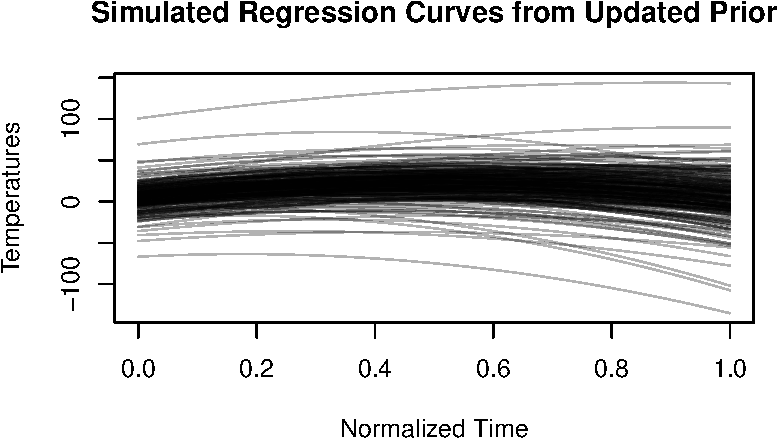
\includegraphics[keepaspectratio]{index_files/figure-pdf/fig-reg-prior-new-1.pdf}}

}

\caption{\label{fig-reg-prior-new}Simulated Regression Curves from
Updated Prior}

\end{figure}%

\subsubsection{4b) Simulating from the
posterior}\label{b-simulating-from-the-posterior}

From the given information, a Gaussian linear regression with a
conjugate prior will have a posterior with the same distribution family.
The following is the joint posterior information.

\[
\beta \mid\sigma^2,y \sim N(\mu_n, \sigma^2 \Omega_n^{-1})
\] \[
\sigma^2\mid y \sim Inv-\chi^2(\nu_n, \sigma^2_n)
\] \[
\Omega_n = X^TX + \Omega_0
\]

\[
\mu_n = \Omega_n^{-1} (X^Ty + \Omega_0\mu_0)
\] \[
\nu_v = \nu_0 +n
\]

\[
\sigma^2_n = (\nu_0\sigma^2_0 + y^Ty + \mu_0^T\Omega_0\mu_0 - \mu_n^T\Omega_n\mu_n) / \nu_n
\] The parameters information from prior and likelihood/model are given,
we can compute the posterior parameters using the following code.

\begin{Shaded}
\begin{Highlighting}[]
\CommentTok{\#settings before simulation}
\NormalTok{time }\OtherTok{=}\NormalTok{ tempLinkoping}\SpecialCharTok{$}\NormalTok{time}
\NormalTok{X }\OtherTok{=} \FunctionTok{cbind}\NormalTok{(}\DecValTok{1}\NormalTok{, time, time}\SpecialCharTok{\^{}}\DecValTok{2}\NormalTok{)}
\NormalTok{y }\OtherTok{=}\NormalTok{ tempLinkoping}\SpecialCharTok{$}\NormalTok{temp}
\NormalTok{n }\OtherTok{=} \FunctionTok{length}\NormalTok{(y)}

\CommentTok{\#beta prior \textasciitilde{} normal updated}
\NormalTok{mu0 }\OtherTok{=} \FunctionTok{c}\NormalTok{(}\DecValTok{5}\NormalTok{,}\DecValTok{70}\NormalTok{,}\SpecialCharTok{{-}}\DecValTok{70}\NormalTok{)}
\NormalTok{Omega0 }\OtherTok{=} \FloatTok{0.01}\SpecialCharTok{*}\FunctionTok{diag}\NormalTok{(}\DecValTok{3}\NormalTok{)}

\CommentTok{\#sigma\_sq prior \textasciitilde{} Inv{-}x\^{}2 }
\NormalTok{nu0 }\OtherTok{=} \DecValTok{3}
\NormalTok{sigma0\_sq }\OtherTok{=} \DecValTok{1}

\CommentTok{\#posterior settings}
\NormalTok{Omega\_n }\OtherTok{=} \FunctionTok{t}\NormalTok{(X) }\SpecialCharTok{\%*\%}\NormalTok{ X }\SpecialCharTok{+}\NormalTok{ Omega0}
\NormalTok{mu\_n }\OtherTok{=} \FunctionTok{solve}\NormalTok{(Omega\_n) }\SpecialCharTok{\%*\%}\NormalTok{ (}\FunctionTok{t}\NormalTok{(X) }\SpecialCharTok{\%*\%}\NormalTok{ y }\SpecialCharTok{+}\NormalTok{ Omega0 }\SpecialCharTok{\%*\%}\NormalTok{ mu0)}
\NormalTok{nu\_n }\OtherTok{=}\NormalTok{ nu0 }\SpecialCharTok{+}\NormalTok{ n}
\NormalTok{sigma\_n\_sq }\OtherTok{=}\NormalTok{ (nu0}\SpecialCharTok{*}\NormalTok{sigma0\_sq }\SpecialCharTok{+} \FunctionTok{t}\NormalTok{(y)}\SpecialCharTok{\%*\%}\NormalTok{y }\SpecialCharTok{+} \FunctionTok{t}\NormalTok{(mu0)}\SpecialCharTok{\%*\%}\NormalTok{Omega0}\SpecialCharTok{\%*\%}\NormalTok{mu0 }\SpecialCharTok{{-}} \FunctionTok{t}\NormalTok{(mu\_n)}\SpecialCharTok{\%*\%}\NormalTok{Omega\_n}\SpecialCharTok{\%*\%}\NormalTok{mu\_n) }\SpecialCharTok{/}\NormalTok{ nu\_n}
\end{Highlighting}
\end{Shaded}

After computing the posterior parameters, we can simulate samples from
the posterior of \(\sigma^2\). Then, the simulated samples of
\(\sigma^2\) can be plugged into \(\beta\mid\sigma^2\) 's posterior
distribution, which is multivariate normal. Finally, we can draw samples
from \(\beta\) 's posterior distribution and visualize the marginal
posteriors of each parameter using histograms as shown in
Figure~\ref{fig-para-hist}.

\begin{Shaded}
\begin{Highlighting}[]
\NormalTok{m }\OtherTok{=} \DecValTok{10000}
\NormalTok{sigma\_sq\_post\_draws }\OtherTok{=} \FunctionTok{rScaledInvChi2}\NormalTok{(m, nu\_n, sigma\_n\_sq)}
\CommentTok{\#store betas draws}
\NormalTok{beta\_post\_draws }\OtherTok{=} \FunctionTok{matrix}\NormalTok{(}\ConstantTok{NA}\NormalTok{, }\AttributeTok{nrow=}\NormalTok{m, }\AttributeTok{ncol=}\FunctionTok{ncol}\NormalTok{(X))}

\ControlFlowTok{for}\NormalTok{ (i }\ControlFlowTok{in} \DecValTok{1}\SpecialCharTok{:}\NormalTok{m)\{}
\NormalTok{  sigma\_sq\_post\_i }\OtherTok{=}\NormalTok{ sigma\_sq\_post\_draws[i]}
\NormalTok{  beta\_post\_var }\OtherTok{=}\NormalTok{ sigma\_sq\_post\_i }\SpecialCharTok{*} \FunctionTok{solve}\NormalTok{(Omega\_n)}
  
\NormalTok{  beta\_post\_draws[i, ] }\OtherTok{=} \FunctionTok{rmvnorm}\NormalTok{(}\DecValTok{1}\NormalTok{, }\AttributeTok{mean=}\FunctionTok{as.vector}\NormalTok{(mu\_n), }\AttributeTok{sigma=}\NormalTok{beta\_post\_var)}
\NormalTok{\}}

\FunctionTok{par}\NormalTok{(}\AttributeTok{mfrow =} \FunctionTok{c}\NormalTok{(}\DecValTok{2}\NormalTok{, }\DecValTok{2}\NormalTok{))}
\NormalTok{beta\_names }\OtherTok{=} \FunctionTok{expression}\NormalTok{(beta[}\DecValTok{0}\NormalTok{], beta[}\DecValTok{1}\NormalTok{], beta[}\DecValTok{2}\NormalTok{])}
\NormalTok{beta\_mains }\OtherTok{=}\FunctionTok{c}\NormalTok{(}\StringTok{"Intercept"}\NormalTok{, }\StringTok{"Time"}\NormalTok{, }\StringTok{"Time\^{}2"}\NormalTok{)}

\ControlFlowTok{for}\NormalTok{ (i }\ControlFlowTok{in} \DecValTok{1}\SpecialCharTok{:}\FunctionTok{length}\NormalTok{(beta\_names))\{}
  \FunctionTok{hist}\NormalTok{(beta\_post\_draws[, i], }\AttributeTok{main=}\NormalTok{beta\_mains[i], }\AttributeTok{xlab=}\NormalTok{beta\_names[i],}
       \AttributeTok{col=}\StringTok{"skyblue"}\NormalTok{,}
       \AttributeTok{freq=}\ConstantTok{FALSE}\NormalTok{)}
\NormalTok{\}}

\FunctionTok{hist}\NormalTok{(sigma\_sq\_post\_draws, }\AttributeTok{main=}\StringTok{"Variance"}\NormalTok{, }\AttributeTok{xlab=}\FunctionTok{expression}\NormalTok{(sigma}\SpecialCharTok{\^{}}\DecValTok{2}\NormalTok{), }\AttributeTok{col=}\StringTok{"skyblue"}\NormalTok{, }\AttributeTok{freq=}\ConstantTok{FALSE}\NormalTok{)}
\end{Highlighting}
\end{Shaded}

\begin{figure}[H]

\centering{

\pandocbounded{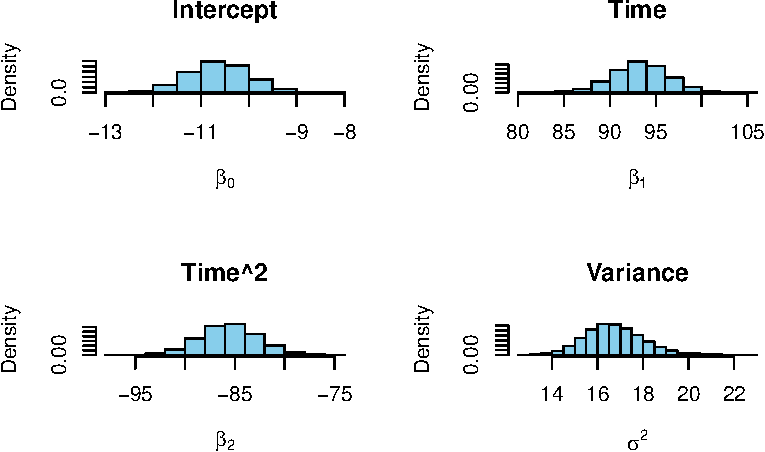
\includegraphics[keepaspectratio]{index_files/figure-pdf/fig-para-hist-1.pdf}}

}

\caption{\label{fig-para-hist}Marginal Distribution of Parameters}

\end{figure}%

Since the marginal posterior distributions of coefficients
\(\beta = (\beta_0, \beta_1, \beta_3)\) are known, the posterior
distribution of the regression function can be computed by plugging the
simulated \(\beta\) posterior draws into the regression model: \[
f(time) = \beta_0 + \beta_1 * time + \beta_2 * time^2
\] After the posterior distribution of the regression function is known,
we can simply compute the posterior median and the equal-tail 95\%
confidence interval for the regression at each time point.
Figure~\ref{fig-reg-post-median} contains the data point from Linkoping
dataset and a posterior median curve of the regression function with
equal-tail 95\% confidence interval.

\begin{Shaded}
\begin{Highlighting}[]
\CommentTok{\# Predictive curves}
\NormalTok{time\_grid }\OtherTok{=}\NormalTok{ tempLinkoping}\SpecialCharTok{$}\NormalTok{time}
\NormalTok{X\_grid }\OtherTok{=} \FunctionTok{cbind}\NormalTok{(}\DecValTok{1}\NormalTok{, time, time}\SpecialCharTok{\^{}}\DecValTok{2}\NormalTok{)}
\CommentTok{\# X\_grid: 366x3, beta\_post\_draws: 10000x3, transpose to 3x10000}
\NormalTok{f\_post }\OtherTok{=}\NormalTok{ X\_grid }\SpecialCharTok{\%*\%} \FunctionTok{t}\NormalTok{(beta\_post\_draws)}

\NormalTok{f\_median }\OtherTok{=} \FunctionTok{apply}\NormalTok{(f\_post, }\DecValTok{1}\NormalTok{, median)}
\NormalTok{f\_lower }\OtherTok{\textless{}{-}} \FunctionTok{apply}\NormalTok{(f\_post, }\DecValTok{1}\NormalTok{, quantile, }\AttributeTok{probs =} \FloatTok{0.025}\NormalTok{)}
\NormalTok{f\_upper }\OtherTok{\textless{}{-}} \FunctionTok{apply}\NormalTok{(f\_post, }\DecValTok{1}\NormalTok{, quantile, }\AttributeTok{probs =} \FloatTok{0.975}\NormalTok{)}

\CommentTok{\# Base R plot version of predictive regression curve}

\CommentTok{\# Set up base plot}
\FunctionTok{plot}\NormalTok{(time\_grid, f\_median, }\AttributeTok{type =} \StringTok{"l"}\NormalTok{, }\AttributeTok{lwd =} \DecValTok{2}\NormalTok{, }\AttributeTok{col =} \StringTok{"red"}\NormalTok{,}
     \AttributeTok{ylim =} \FunctionTok{range}\NormalTok{(}\FunctionTok{c}\NormalTok{(f\_lower, f\_upper, y)),}
     \AttributeTok{xlab =} \StringTok{"Normalized Time"}\NormalTok{, }\AttributeTok{ylab =} \StringTok{"Temperature"}\NormalTok{,}
     \AttributeTok{main =} \StringTok{"Posterior Median of Regression Curve with 95\% C.I"}\NormalTok{)}

\CommentTok{\# Add credible interval (ribbon)}
\FunctionTok{polygon}\NormalTok{(}\FunctionTok{c}\NormalTok{(time\_grid, }\FunctionTok{rev}\NormalTok{(time\_grid)),}
        \FunctionTok{c}\NormalTok{(f\_lower, }\FunctionTok{rev}\NormalTok{(f\_upper)),}
        \AttributeTok{col =} \FunctionTok{rgb}\NormalTok{(}\DecValTok{70}\SpecialCharTok{/}\DecValTok{255}\NormalTok{, }\DecValTok{130}\SpecialCharTok{/}\DecValTok{255}\NormalTok{, }\DecValTok{180}\SpecialCharTok{/}\DecValTok{255}\NormalTok{, }\FloatTok{0.4}\NormalTok{), }\AttributeTok{border =} \ConstantTok{NA}\NormalTok{)}

\CommentTok{\# Add observed data points}
\FunctionTok{points}\NormalTok{(time, y, }\AttributeTok{pch =} \DecValTok{20}\NormalTok{, }\AttributeTok{col =} \StringTok{"gray40"}\NormalTok{)}

\CommentTok{\# Optionally add median line again (drawn over ribbon)}
\FunctionTok{lines}\NormalTok{(time\_grid, f\_median, }\AttributeTok{col =} \StringTok{"red"}\NormalTok{, }\AttributeTok{lwd =} \DecValTok{2}\NormalTok{)}
\end{Highlighting}
\end{Shaded}

\begin{figure}[H]

\centering{

\pandocbounded{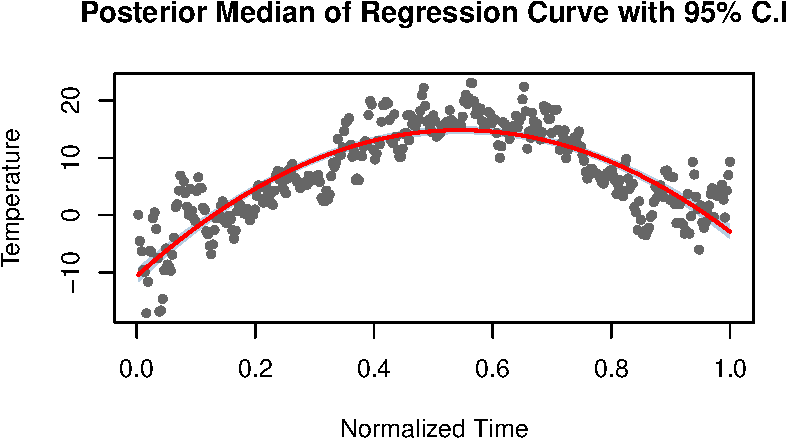
\includegraphics[keepaspectratio]{index_files/figure-pdf/fig-reg-post-median-1.pdf}}

}

\caption{\label{fig-reg-post-median}Posterior Median of Regression Curve
with 95\% C.I}

\end{figure}%

From the posterior median of the regression curve, we can clearly
confirm that the 95\% confidence interval band does not contain all the
observed data point, because the confidence interval band only reflect
the uncertainty of the posterior median regression function without the
noise term \(\epsilon \sim N(0, \sigma^2)\). Therefore, it is not
necessary for the confidence interval band of the regression function to
include every data points.

\subsubsection{4c) Locating the day with the highest expected
temperature}\label{c-locating-the-day-with-the-highest-expected-temperature}

Given the highest expected temperature at each time point \(x_{max}\):

\[
x_{max} = -\frac{\beta_1}{2\beta_2}
\] Since the posterior distribution of \(\beta\) is known from previous
problem, we can use the samples from the distribution to compute the
values of \(x_{max}\) at each time point, and the values can be
visualized through a histogram as shown in Figure~\ref{fig-xmax-hist}.

\begin{Shaded}
\begin{Highlighting}[]
\NormalTok{beta1\_post\_samples }\OtherTok{=}\NormalTok{ beta\_post\_draws[, }\DecValTok{2}\NormalTok{]}
\NormalTok{beta2\_post\_samples }\OtherTok{=}\NormalTok{ beta\_post\_draws[, }\DecValTok{3}\NormalTok{]}

\NormalTok{x\_max }\OtherTok{=} \SpecialCharTok{{-}}\NormalTok{beta1\_post\_samples }\SpecialCharTok{/}\NormalTok{ (}\DecValTok{2}\SpecialCharTok{*}\NormalTok{beta2\_post\_samples)}

\FunctionTok{par}\NormalTok{(}\AttributeTok{mfrow=}\FunctionTok{c}\NormalTok{(}\DecValTok{1}\NormalTok{, }\DecValTok{2}\NormalTok{))}

\FunctionTok{hist}\NormalTok{(x\_max, }\AttributeTok{breaks=}\DecValTok{50}\NormalTok{, }\AttributeTok{freq =} \ConstantTok{FALSE}\NormalTok{, }\AttributeTok{col=}\StringTok{"lightblue"}\NormalTok{,}
     \AttributeTok{main=}\StringTok{"Posterior of x\_max"}\NormalTok{,}
     \AttributeTok{xlab=}\StringTok{"Time With Highest Expected Temperature"}\NormalTok{)}

\CommentTok{\#unnormalized time to regular day}
\FunctionTok{hist}\NormalTok{(x\_max}\SpecialCharTok{*}\DecValTok{366}\NormalTok{, }\AttributeTok{breaks=}\DecValTok{50}\NormalTok{, }\AttributeTok{freq =} \ConstantTok{FALSE}\NormalTok{, }\AttributeTok{col=}\StringTok{"steelblue"}\NormalTok{,}
     \AttributeTok{main=}\StringTok{"Posterior of x\_max"}\NormalTok{,}
     \AttributeTok{xlab=}\StringTok{"Day With Highest Expected Temperature"}\NormalTok{)}
\end{Highlighting}
\end{Shaded}

\begin{figure}[H]

\centering{

\pandocbounded{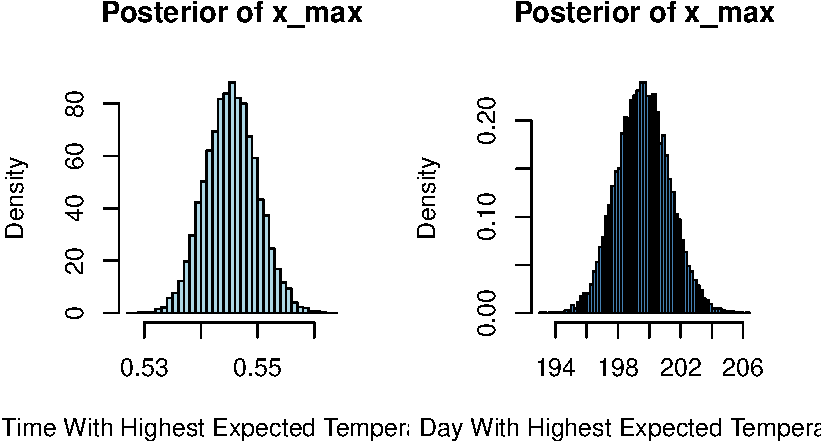
\includegraphics[keepaspectratio]{index_files/figure-pdf/fig-xmax-hist-1.pdf}}

}

\caption{\label{fig-xmax-hist}Posterior of x\_max}

\end{figure}%




\end{document}
